\documentclass{beamer}

\mode<presentation>
{
\usetheme{Warsaw}

\setbeamercovered{transparent}
}

\usepackage[english]{babel}
\usepackage[latin1]{inputenc}
\usepackage{graphicx}

\usepackage{mathptmx}
\usepackage[scaled=.90]{helvet}
\usepackage{courier}


\usepackage[T1]{fontenc}


\title{}

\author{Salman A. Khokhar}

\institute{%
Honda Research Institute\\
}

\date{\today}

\subject{Internship Talk}

\AtBeginSubsection[]
{
\begin{frame}<beamer>
\frametitle{Outline}
\tableofcontents[currentsection,currentsubsection]
\end{frame}
}

% If you wish to uncover everything in a step-wise fashion, uncomment
% the following command:

%\beamerdefaultoverlayspecification{<+->}

\begin{document}

\begin{frame}
\titlepage
\end{frame}

\begin{frame}
\frametitle{Outline}
\tableofcontents
% You might wish to add the option [pausesections]
\end{frame}


\section{Introduction}

\begin{frame}
\frametitle{Problem Description}

\begin{itemize}
  \item Risk assessment at intersections
  \item Prediction of future paths of observed vehicles
\end{itemize}
\end{frame}

\section{Scenario and Method}

\begin{frame}
\frametitle{Setting}

\begin{itemize}
  \item At an intersection:
  \begin{itemize}
    \item Observe other vehicles at other ends of the intersection
    \item Estimate their GPS position
    \item Compyte features using map data
    \item Make a prediction about their future behavior
  \end{itemize}
\end{itemize}
\end{frame}

\begin{frame}
\frametitle{Setting}
An ideal scenario:
\begin{itemize}
  \item V2V communication between our vehicle and observed vehicles
  \item Transfer of GPS position information
\end{itemize}
Our setting:
\begin{itemize}
  \item unavailable: V2V communication
  \item available: High precision GPS unit
  \item Experimental setting assumptions:
  \begin{itemize}
    \item The vehicle with a GPS unit is the 'observed' vehicle
    \item Data from the observed vehicle is transferred to us
    \item We have to predict future behavior of the driven vehicle
   	\item Our own vehicle is at the same intersection, but
   	\item Our exact position is irrelevant for the prediction
   \end{itemize}
\end{itemize}
\end{frame}

\begin{frame}
\frametitle{Data collection}
	Required data:
	\begin{itemize}
	\item Map information
	\item High precision GPS information
	\end{itemize}
	Available options:
	\begin{itemize}
	   \item KITTI dataset and open street maps
	   \item Zenrin and our own collected data 
	\end{itemize}
\end{frame}

\begin{frame}
\frametitle{Data collection}
	
	 \begin{figure}
 		\centering
    	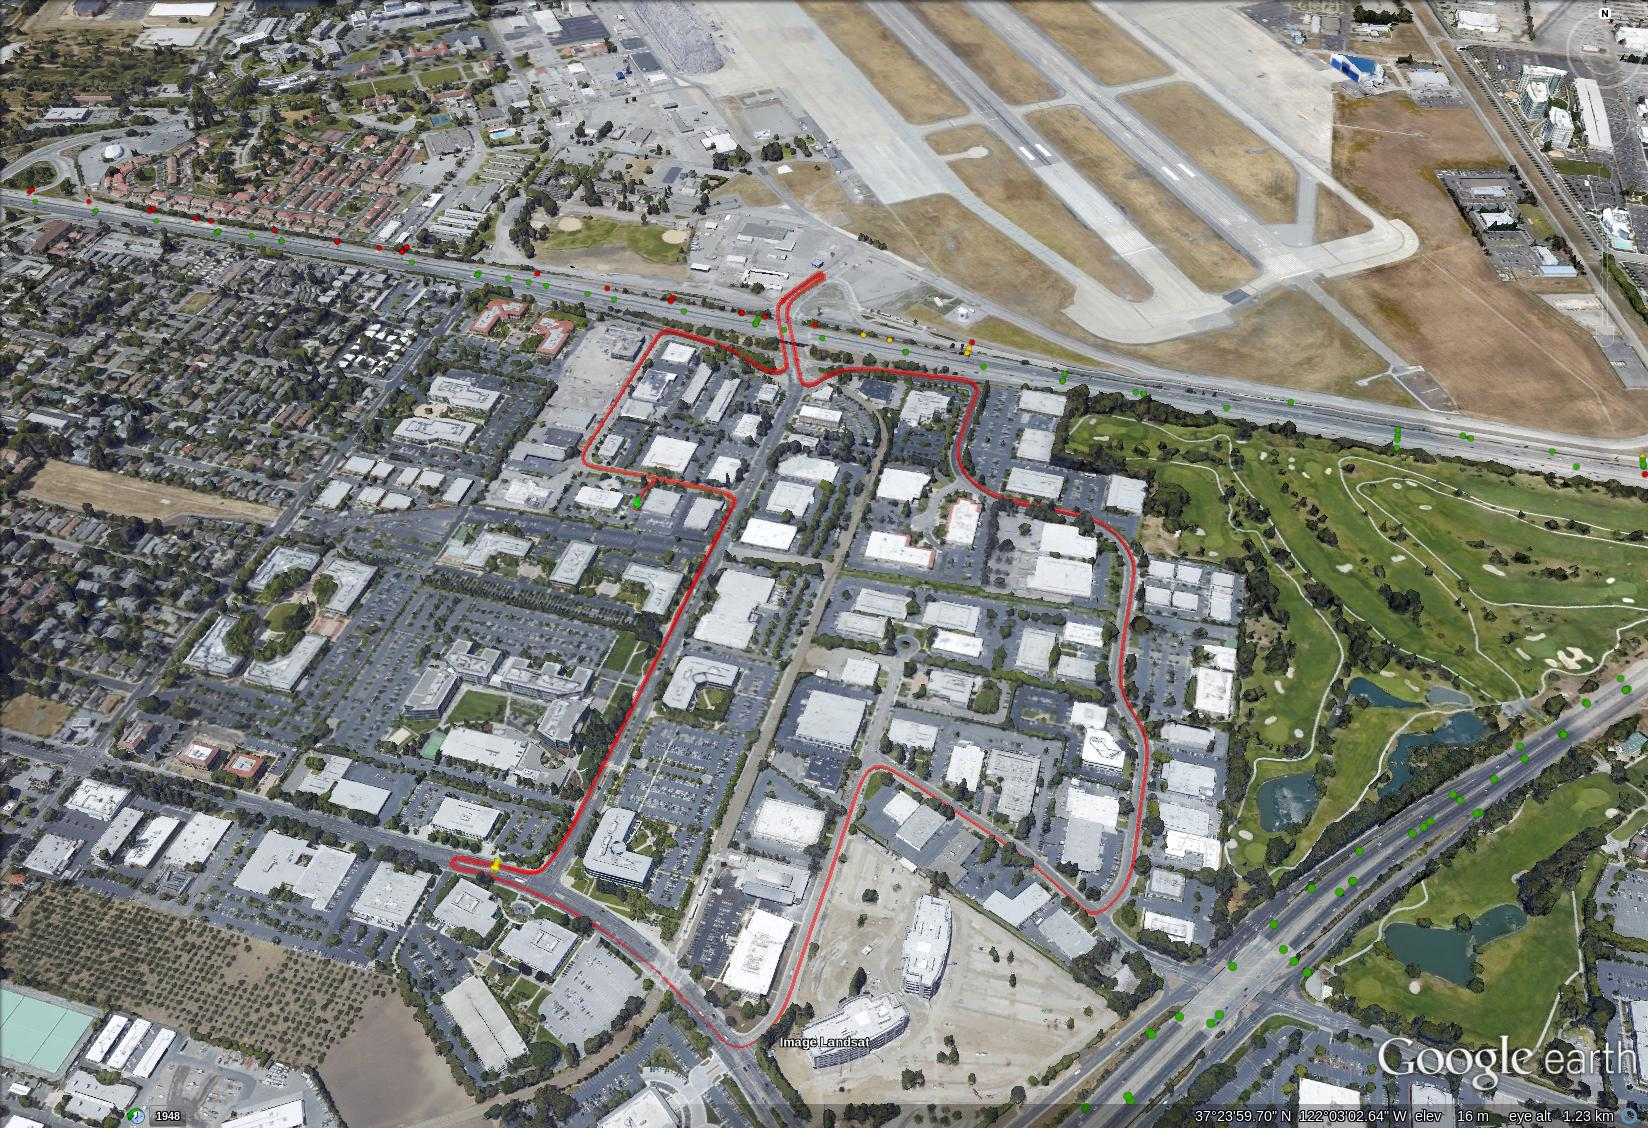
\includegraphics[width =
    	0.9\textwidth]{./presentation_files/dataCollection[061714].jpg}
    	\caption{Awesome figure}
	\end{figure}
	
\end{frame}

\begin{frame}
\frametitle{Data collection}
	
	 \begin{figure}
 		\centering
    	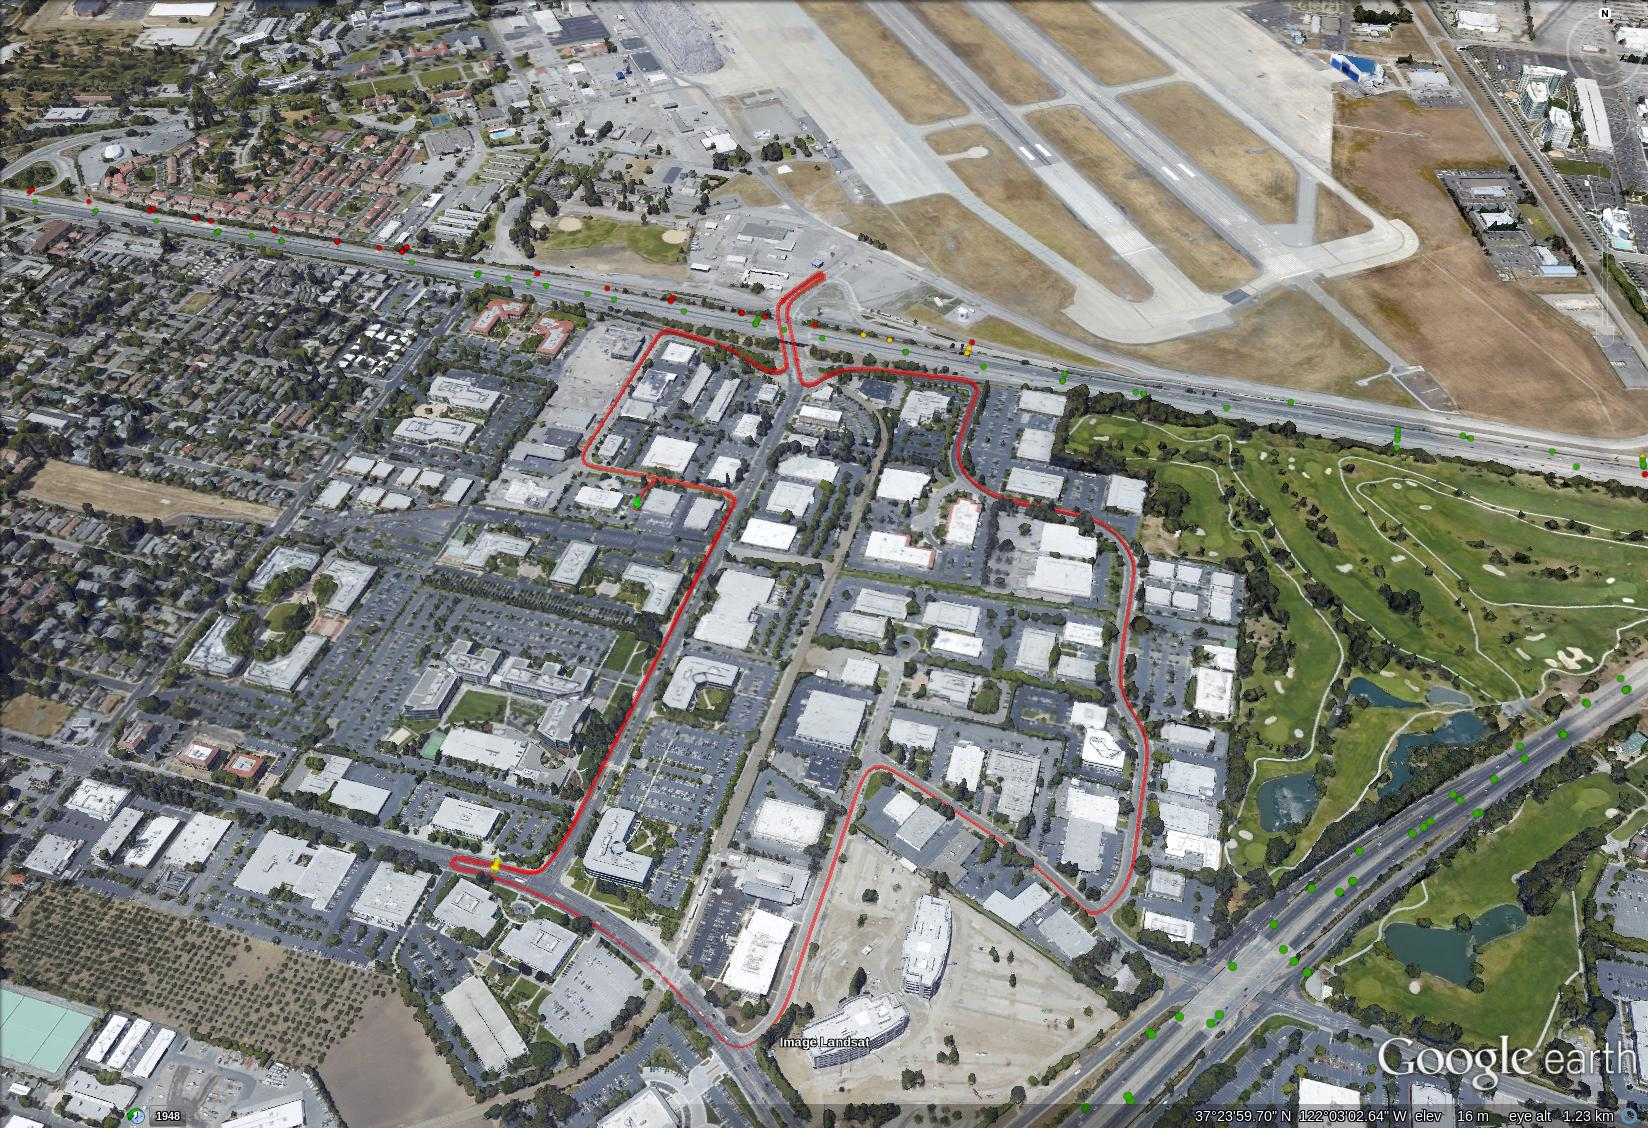
\includegraphics[width =
    	0.9\textwidth]{./presentation_files/dataCollection[061714].eps}
    	\caption{Awesome figure}
	\end{figure}
	
\end{frame}

\begin{frame}
\frametitle{Features}
	Available information:
	\begin{itemize}
	\item Vehicle pose from the CAN bus
	\begin{itemize}\item only latitude and longitude are used \end{itemize}
	\item Zenrin map data
	\end{itemize}
	Features computed:
	\begin{itemize}
	   \item Distance from lane center
	   \item Distance from intersection
	   \item Angle between lane orientation and vehicle heading
	\end{itemize}
\end{frame}

\begin{frame}
\frametitle{Track pre-processing}
	We get continuous GPS track from one drive
	\begin{itemize}
	\item Tracks are clipped at a specified distance from intersection centers
	\item Stops are detected and removed before model learning or testing
	\end{itemize}
	% show example video of track with and without stop (on GmapsFX GUI)
	
\end{frame}

\begin{frame}
\frametitle{Learning model}
	\begin{itemize}
	  \item A time series of vector data
	  \begin{itemize}
	    \item time series may be of unequal lengths due to:
	    \begin{itemize}
	      \item stops
	      \item unequal velocity
	      \item intersection structure
	      \end{itemize}
	      \end{itemize}
	  \item Event classes
	  \begin{itemize}
	    \item Left turn
	    \item Right turn
	    \item Straight
	   \end{itemize}
	   \item Train a hidden markov model for each event
	   \item Compute probabilities at test time from trained models
	\end{itemize}
\end{frame}

\section{Experiments and Results}
\subsection[HMM]{Hidden Markov Models}
\begin{frame}
\frametitle{HMM training}
	\begin{itemize}
	  \item Feature computation
	  \begin{itemize}
	    \item Begins 15 meters from intersection
	    \item Ends 15 meters into intersection
	   \end{itemize}
	   \item Separate HMM model trained for each event class
	   \item Each model trained using a single gaussian per feature per state
	   \item All gaussians initialized to large variances with zero means
	   \item Training performed using a 80-20 split
	  \item  
	\end{itemize}
\end{frame}

\begin{frame}

\frametitle{HMM classification performance}
% insert plot of HMM performance over distance	

\end{frame}

\begin{frame}

\frametitle{Feature comparison}
% insert plot of HMM using individual features or combinations
 	\begin{figure}
 		\centering
    	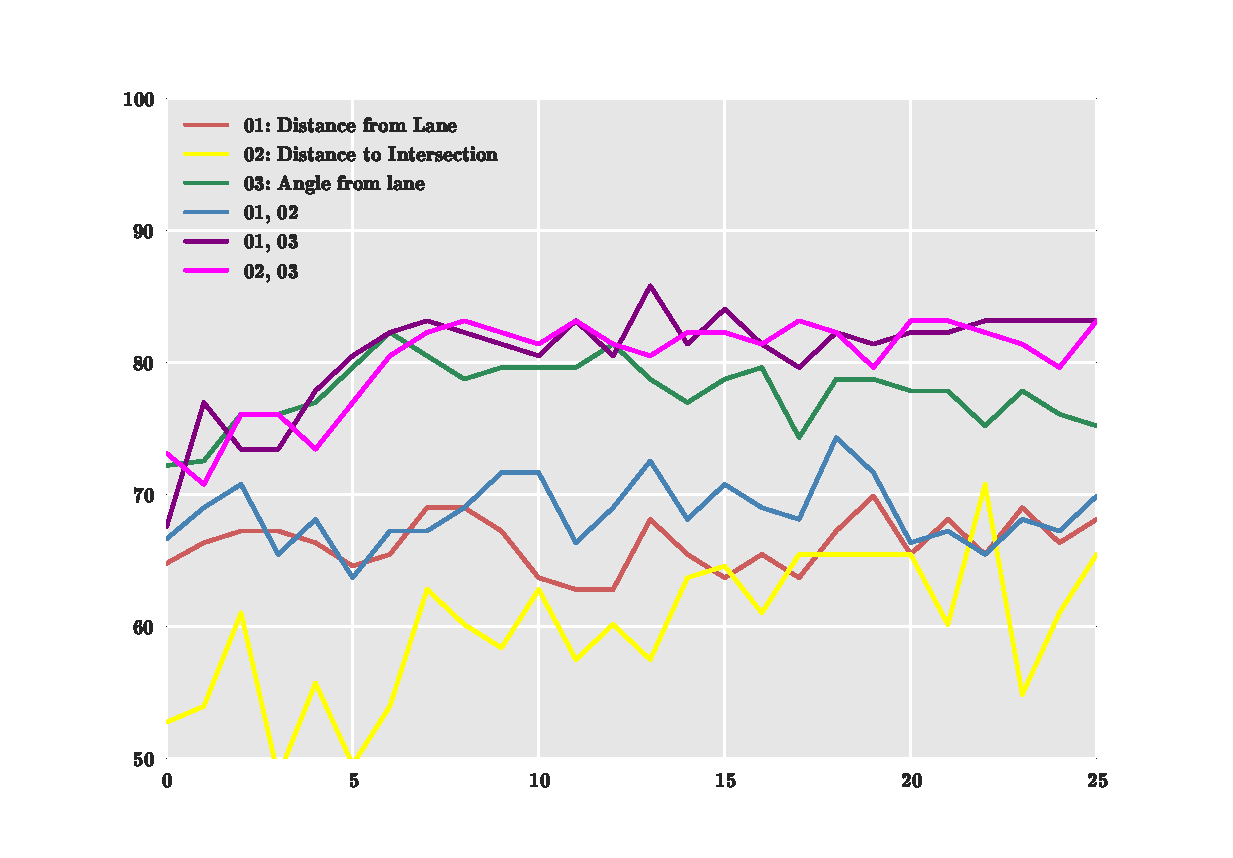
\includegraphics[width =
    	0.9\textwidth]{./presentation_files/feature_comparison.eps}
    	\caption{Awesome figure}
	\end{figure}

\end{frame}

\begin{frame}

\frametitle{Hidden states}
	\begin{figure}
 		\centering
    	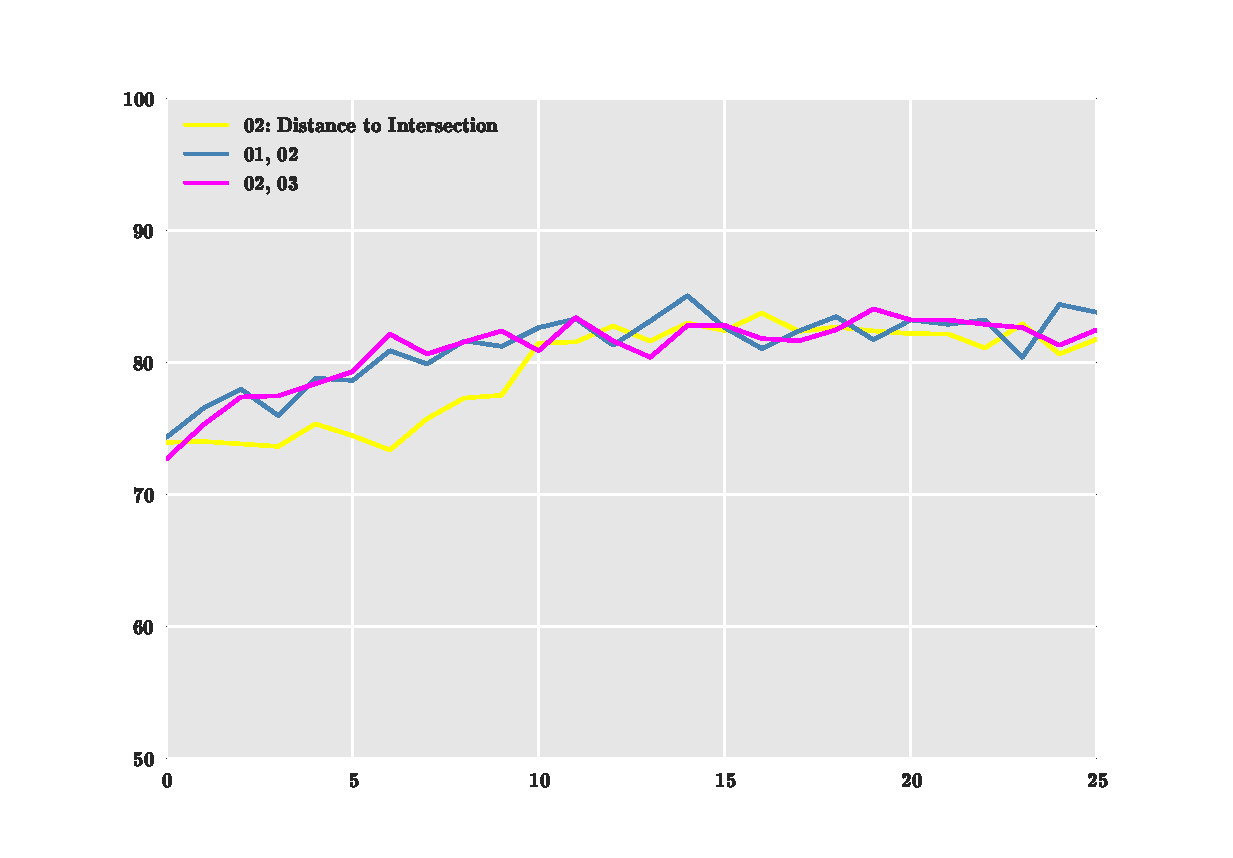
\includegraphics[width =
    	0.9\textwidth]{./presentation_files/hmm_state_comparison.eps}
    	\caption{Awesome figure}
	\end{figure}
\end{frame}



\begin{frame}

\frametitle{Event confusion}
% show confusion matrices	

\end{frame}

\begin{frame}

\frametitle{Demo video}
% show video of GUI or switch over to demo	

\end{frame}

\subsection[Comparisons]{Comparisons}
\begin{frame}
\frametitle{Performance comparison}
% insert plot of HMM performance over distance	
\begin{itemize}
  \item Rule based decision (baseline)
  \item SVM
\end{itemize}

\end{frame}

\section{Summary}
\begin{frame}
	Conclusions:
	\begin{itemize}
	  \item HMM prediction with given features caps at ~85-88 \%
	  \item Multi-modal HMM prediction may improve learning
	  \item We are trying a Dynamic Bayesian Network to improve performance
	\end{itemize}
\end{frame}

\end{document}
